\documentclass[a4paper,12pt]{article}

% ===================================================================
% PACKAGE IMPORTS
% ===================================================================
\usepackage[utf8]{inputenc}
\usepackage[T5]{fontenc}
\usepackage[vietnamese]{babel}
\usepackage{graphicx}  % Để thêm logo
\usepackage{fancyhdr}  % Tạo header và footer
\usepackage{geometry}  % Cài đặt lề trang
\usepackage{tikz} 
\usetikzlibrary{positioning}
\usepackage{listings}
\usepackage{xcolor}
\usepackage{float}     % Để sử dụng [H] cho vị trí cố định của hình
\usepackage{amsmath}   % Để hỗ trợ math equations
\usepackage{hyperref}  % Để tạo hyperlink trong mục lục (load cuối cùng)

% ===================================================================
% HYPERREF SETUP
% ===================================================================
\hypersetup{
    colorlinks=true,
    linkcolor=blue,
    filecolor=magenta,      
    urlcolor=cyan,
    pdftitle={Báo cáo đồ án Socket - RTSP/RTP Video Streaming},
    pdfpagemode=FullScreen,
}

% ===================================================================
% CODE LISTING COLORS
% ===================================================================
\definecolor{codegreen}{rgb}{0,0.6,0}
\definecolor{codegray}{rgb}{0.5,0.5,0.5}
\definecolor{codepurple}{rgb}{0.58,0,0.82}
\definecolor{backcolour}{rgb}{0.95,0.95,0.92}

% ===================================================================
% LISTING STYLE FOR PYTHON CODE
% ===================================================================
\lstdefinestyle{pythonstyle}{
    backgroundcolor=\color{backcolour},   
    commentstyle=\color{codegreen},
    keywordstyle=\color{magenta},
    numberstyle=\tiny\color{codegray},
    stringstyle=\color{codepurple},
    basicstyle=\ttfamily\small,
    breakatwhitespace=false,         
    breaklines=true,                 
    keepspaces=true,                 
    numbers=left,                    
    numbersep=5pt,                  
    showspaces=false,                
    showstringspaces=false,
    showtabs=false,                  
    tabsize=4
}

\lstset{style=pythonstyle}

% ===================================================================
% HEADER/FOOTER SETUP
% ===================================================================
\lhead{Học phần: Mạng máy tính}
\rhead{Trường Đại học Khoa học Tự nhiên}
\cfoot{Trang \thepage}

% ===================================================================
% PAGE GEOMETRY
% ===================================================================
\geometry{top=2cm, bottom=2cm, left=2.5cm, right=2.5cm}
\setlength{\headheight}{15pt}
\renewcommand{\contentsname}{\huge Mục lục}

% ===================================================================
% BEGIN DOCUMENT
% ===================================================================
\begin{document}

% ===================================================================
% IMPORT SECTION FILES
% 
% Hướng dẫn cho team:
% - Mỗi thành viên làm việc trên file riêng trong thư mục sections/
% - File chính này CHỈ import các section files
% - Không chỉnh sửa nội dung section trong file này
% 
% Phân công:
% - 0_trang_bia.tex: Trang bìa và mục lục
% - 1_thong_tin.tex: Thông tin nhóm và tổng quan dự án
% - 2_rtsp_rtp.tex: RTSP/RTP cơ bản (4 điểm) - Trần Hoàng Phúc
% - 3_hd_streaming.tex: HD Streaming (3 điểm) - Nguyễn Hữu Gia Minh
% - 4_buffer.tex: Client-Side Buffer (2.5 điểm) - Nguyễn Khánh Linh
% - 5_ket_luan.tex: Kết luận - Team Leader hoặc cả nhóm
% ===================================================================

% Trang bìa và mục lục
\begin{titlepage}
    \centering
    \textbf{TRƯỜNG ĐẠI HỌC KHOA HỌC TỰ NHIÊN} \\[0.5cm]
    \textbf{ĐẠI HỌC QUỐC GIA THÀNH PHỐ HỒ CHÍ MINH} \\[0.5cm]
    \textbf{KHOA CÔNG NGHỆ THÔNG TIN} \\[0.5cm]

    \hrule
    \Huge
    \begin{center}
    \textbf{\huge Báo cáo đồ án thực hành}\\[0.5cm]
    \textbf{\Large Nội dung: Lập trình Socket}
    \end{center}
    \hrule
    \Large
    \begin{center}
    Môn học: Mạng Máy Tính \\
    \end{center}

    \begin{flushleft}
        \textbf{Giáo viên hướng dẫn:} \\
        Thầy Lê Ngọc Sơn \\
        Thầy Nguyễn Thanh Quân \\
    \end{flushleft}

    \begin{flushleft}
        \textbf{Thành viên:} \\
        Nguyễn Hữu Gia Minh - 24127078 \\
        Nguyễn Khánh Linh - 24127197 \\
        Trần Hoàng Phúc - 24127505 \\
    \end{flushleft}

    \vfill

    \begin{center}
        
\includegraphics[width=6cm]{LOGO.png} \\[1cm]
        Ngày 21 tháng 12 năm 2024
    \end{center}
    
    \thispagestyle{empty}  % Đảm bảo không có header/footer trên trang bìa
\end{titlepage}

% Kích hoạt header/footer cho các trang sau trang bìa
\pagestyle{fancy}  % Áp dụng header/footer từ trang tiếp theo

% Chỉnh sửa footer và header cho các trang còn lại
\cfoot{\thepage}  % Footer giữa hiển thị số trang

\newpage
\tableofcontents
\newpage


% Phần 1-2: Thông tin dự án và kiến trúc tổng quan
\section{Thông tin nhóm}
-   Tên học phần: Mạng máy tính. \\
-   Đồ án thực hiện: Lập trình Socket. \\
-   Thời gian thực hiện: 23/11/2025 đến ngày 14/12/2025. \\
-   Danh sách thành viên: \\
\begin{table}[h!]
\centering
\begin{tabular}{|c|c|l|l|}
\hline
\textbf{STT} & \textbf{MSSV} & \textbf{Họ và tên} & \textbf{Vai trò} \\ \hline
01           & 23127004      & Nguyễn Khánh Linh        & Thành viên      \\ \hline
02           & 23127113      & Trần Hoàng Phúc & Nhóm trưởng    \\ \hline
03           & 23127165      & Nguyễn Hữu Gia Minh     & Thành viên      \\ \hline
\end{tabular}
\end{table}

\section{Thông tin đồ án}

\subsection{Tổng quan đồ án}
\begin{itemize}
    \item \textbf{Yêu cầu:} Xây dựng một hệ thống trình phát video trực tuyến gồm client và server, sử dụng:
    \begin{itemize}
        \item \textbf{RTSP (Real-Time Streaming Protocol):} Giao thức điều khiển trên TCP
        \item \textbf{RTP (Real-time Transport Protocol):} Giao thức truyền dữ liệu media trên UDP
    \end{itemize}
    \item \textbf{Mục đích:} Hiểu rõ về các giao thức mạng thời gian thực, quản lý trạng thái phiên kết nối, và kỹ thuật đóng gói (packetization) dữ liệu đa phương tiện.
\end{itemize}

\subsection{Mục tiêu}
\begin{itemize}
    \item Triển khai giao thức RTSP phía client để gửi các lệnh điều khiển (SETUP, PLAY, PAUSE, TEARDOWN).
    \item Triển khai RTP packetization phía server để gửi video dạng MJPEG tới client.
    \item Hiểu và quản lý trạng thái phiên RTSP.
    \item Hỗ trợ HD Video Streaming và Client-Side Caching để cải thiện chất lượng phát video.
\end{itemize}

\subsection{Kiến trúc hệ thống}

\subsubsection{Kênh điều khiển (RTSP)}
\begin{itemize}
    \item Sử dụng TCP để truyền các lệnh RTSP.
    \item Port mặc định: 554 (TCP).
    \item Client gửi các lệnh:
    \begin{itemize}
        \item \textbf{SETUP:} Thiết lập phiên kết nối và thông số transport.
        \item \textbf{PLAY:} Bắt đầu phát video.
        \item \textbf{PAUSE:} Tạm dừng phát video.
        \item \textbf{TEARDOWN:} Kết thúc phiên kết nối.
    \end{itemize}
    \item Mỗi lệnh RTSP phải kèm CSeq header (số thứ tự lệnh) và Session header (mã phiên) nếu cần.
\end{itemize}

\subsubsection{Kênh dữ liệu (RTP)}
\begin{itemize}
    \item Sử dụng UDP để truyền dữ liệu video.
    \item Server thực hiện RTP packetization:
    \begin{itemize}
        \item Header gồm các trường: V, P, X, CC, M, PT, Sequence Number, Timestamp, SSRC.
        \item Payload là dữ liệu video MJPEG.
    \end{itemize}
    \item Client nhận RTP packet và giải mã để hiển thị video.
\end{itemize}

\subsubsection{Client}
\begin{itemize}
    \item Client cần triển khai hành vi khi người dùng nhấn các nút điều khiển:
    \begin{itemize}
        \item Mở kết nối RTSP với server khi khởi động.
        \item Gửi và nhận các lệnh RTSP.
        \item Quản lý trạng thái phiên (INIT, READY, PLAYING).
        \item Nhận và hiển thị dữ liệu RTP.
    \end{itemize}
\end{itemize}

\subsubsection{Server}
\begin{itemize}
    \item Server đọc video MJPEG từ file và gửi từng frame dưới dạng RTP packet.
    \item Server phản hồi tất cả các lệnh RTSP từ client (200 OK, 404 FILE\_NOT\_FOUND, 500 CONNECTION\_ERROR).
    \item RTP packetization:
    \begin{itemize}
        \item V = 2, P = X = CC = M = 0, PT = 26 (MJPEG), Sequence Number theo frame, Timestamp từ Python time module, SSRC tự chọn.
    \end{itemize}
\end{itemize}

\subsection{Yêu cầu kỹ thuật}

\subsubsection{PHẦN 1: Triển khai Client}

\paragraph{A. Các Module}
\begin{itemize}
    \item \textbf{ClientLauncher:} Khởi động giao diện người dùng (không cần sửa)
    \item \textbf{Client:} Xử lý logic RTSP (cần hoàn thiện)
\end{itemize}

\paragraph{B. Triển Khai RTSP Commands}

\paragraph{1. Lệnh SETUP}
\begin{itemize}
    \item \textbf{Mục đích:} Thiết lập phiên làm việc và tham số truyền tải
    \item \textbf{Công việc cần làm:}
    \begin{itemize}
        \item Tạo UDP socket để nhận dữ liệu RTP từ Server
        \item Thiết lập timeout = 0.5 giây cho socket
        \item Gửi RTSP request đến Server:
        \begin{itemize}
            \item CSeq: Số thứ tự lệnh (bắt đầu từ 1)
            \item Transport: RTP/UDP; client\_port=<RTP\_port>
        \end{itemize}
        \item Nhận response từ server
        \item Parse Session ID từ header response để sử dụng cho các lệnh sau
    \end{itemize}
\end{itemize}

\paragraph{2. Lệnh PLAY}
\begin{itemize}
    \item \textbf{Mục đích:} Bắt đầu phát video
    \item \textbf{Công việc cần làm:}
    \begin{itemize}
        \item Gửi request PLAY với headers:
        \begin{itemize}
            \item CSeq: Tăng lên 1 so với lệnh trước
            \item Session: Session ID nhận được từ SETUP
            \item KHÔNG có Transport header
        \end{itemize}
        \item Nhận và xử lý response từ server
        \item Cập nhật trạng thái client sang PLAYING
    \end{itemize}
\end{itemize}

\paragraph{3. Lệnh PAUSE}
\begin{itemize}
    \item \textbf{Mục đích:} Tạm dừng phát video
    \item \textbf{Công việc cần làm:}
    \begin{itemize}
        \item Gửi request PAUSE với headers:
        \begin{itemize}
            \item CSeq: Tăng lên 1
            \item Session: Session ID
            \item KHÔNG có Transport header
        \end{itemize}
        \item Nhận response
        \item Cập nhật trạng thái client sang READY
    \end{itemize}
\end{itemize}

\paragraph{4. Lệnh TEARDOWN}
\begin{itemize}
    \item \textbf{Mục đích:} Kết thúc phiên và đóng kết nối
    \item \textbf{Công việc cần làm:}
    \begin{itemize}
        \item Gửi request TEARDOWN với headers:
        \begin{itemize}
            \item CSeq: Tăng lên 1
            \item Session: Session ID
            \item KHÔNG có Transport header
        \end{itemize}
        \item Nhận response
        \item Đóng socket và cập nhật trạng thái về INIT
    \end{itemize}
\end{itemize}

\textbf{C. Định Dạng RTSP Message}

\begin{itemize}
    \item \textbf{Request Format:}
    \begin{verbatim}
<METHOD> <video_file> RTSP/1.0
CSeq: <sequence_number>
[Session: <session_id>]
[Transport: RTP/UDP; client_port=<port>]
    \end{verbatim}
    
    \item \textbf{Response Format:}
    \begin{verbatim}
RTSP/1.0 <status_code> <status_message>
CSeq: <sequence_number>
Session: <session_id>
    \end{verbatim}
    
    \item \textbf{Mã trạng thái:}
    \begin{itemize}
        \item 200: Thành công
        \item 404: File không tìm thấy
        \item 500: Lỗi kết nối
    \end{itemize}
\end{itemize}

\begin{figure}[H]
\centering
\begin{tikzpicture}[
    state/.style={rectangle, draw, minimum width=2cm, minimum height=1cm, align=center},
    arrow/.style={->, thick}
]
    \node[state] (init1) {INIT};
    \node[state, below=2cm of init1] (ready) {READY};
    \node[state, below=2cm of ready] (playing) {PLAYING};
    \node[state, below=2cm of playing] (init2) {INIT};
    
    \draw[arrow] (init1) -- node[right] {SETUP} (ready);
    \draw[arrow] (ready) -- node[right] {PLAY} (playing);
    \draw[arrow] (playing) to[bend left=45] node[left] {PAUSE} (ready);
    \draw[arrow] (ready) to[bend left=45] node[right] {} (playing);
    \draw[arrow] (playing) -- node[right] {TEARDOWN} (init2);
\end{tikzpicture}
\caption{RTSP State Machine}
\end{figure}

\begin{figure}[H]
    \centering
    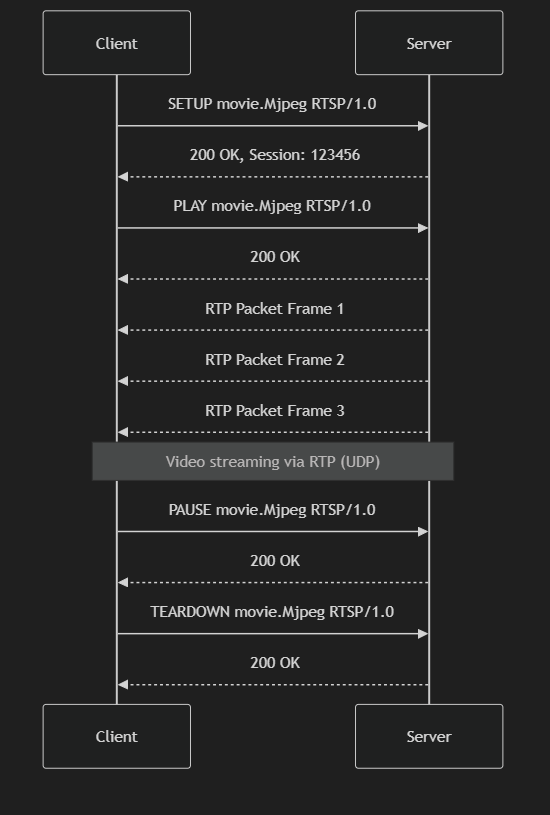
\includegraphics[width=0.8\textwidth]{DIAGRAM1.png}
    \caption{Sơ đồ kiến trúc hệ thống}
\end{figure}

\clearpage


% Phần 3: RTSP/RTP cơ bản (4 điểm) - Trần Hoàng Phúc
% ===================================================================
% PHẦN NÀY DO: Trần Hoàng Phúc phụ trách
% Nội dung: Triển khai RTSP/RTP cơ bản (4 điểm)
% ===================================================================

\section{Triển khai giao thức RTSP ở Client và đóng gói RTP ở Server (4 điểm)}

\textbf{Phần này chỉ bao gồm triển khai CƠ BẢN của giao thức RTSP và RTP, KHÔNG bao gồm các tính năng mở rộng như frame fragmentation cho HD video.}

\subsection{RTSP Protocol - Client Side}

\subsubsection{RTSP State Machine \& Constants}
Client quản lý trạng thái phiên RTSP thông qua state machine với 3 trạng thái chính:

\begin{lstlisting}[language=Python, caption={RTSP State Machine}]
class Client:
    # RTSP States
    INIT = 0      # Trang thai khoi tao
    READY = 1     # San sang phat video
    PLAYING = 2   # Dang phat video
    state = INIT
    
    # RTSP Request Types
    SETUP = 0
    PLAY = 1
    PAUSE = 2
    TEARDOWN = 3
\end{lstlisting}

\textbf{Luồng chuyển trạng thái:}
\begin{itemize}
    \item \texttt{INIT → READY}: Sau khi nhận SETUP response thành công
    \item \texttt{READY → PLAYING}: Sau khi nhận PLAY response thành công
    \item \texttt{PLAYING → READY}: Sau khi nhận PAUSE response thành công
    \item \texttt{READY/PLAYING → INIT}: Sau khi nhận TEARDOWN response thành công
\end{itemize}

\subsubsection{Gửi RTSP Requests}

\paragraph{Hàm sendRtspRequest()}
Hàm này xử lý việc tạo và gửi các RTSP request đến server qua kết nối TCP.

\begin{lstlisting}[language=Python, caption={SETUP Request}]
def sendRtspRequest(self, requestCode):
    """Gui RTSP request den server"""
    request = ""
    
    if requestCode == self.SETUP and self.state == self.INIT:
        # Bat dau thread nhan RTSP responses
        threading.Thread(target=self.recvRtspReply, daemon=True).start()
        
        self.rtspSeq += 1
        # Format: SETUP <filename> RTSP/1.0
        request = f"SETUP {self.fileName} RTSP/1.0\n"
        request += f"CSeq: {self.rtspSeq}\n"
        request += f"Transport: RTP/UDP; client_port={self.rtpPort}"
        self.requestSent = self.SETUP
\end{lstlisting}

\textbf{Chi tiết SETUP Request:}
\begin{itemize}
    \item Khởi tạo thread \texttt{recvRtspReply} để nhận response bất đồng bộ
    \item Tăng \texttt{rtspSeq} để đánh số thứ tự request
    \item Header \texttt{Transport} chỉ định cổng UDP mà client sẽ nhận RTP packets
    \item Lưu loại request đã gửi vào \texttt{requestSent}
\end{itemize}

\begin{lstlisting}[language=Python, caption={PLAY Request}]
elif requestCode == self.PLAY and self.state == self.READY:
    self.rtspSeq += 1
    # Format: PLAY <filename> RTSP/1.0
    request = f"PLAY {self.fileName} RTSP/1.0\n"
    request += f"CSeq: {self.rtspSeq}\n"
    request += f"Session: {self.sessionId}"
    self.requestSent = self.PLAY
\end{lstlisting}

\textbf{Chi tiết PLAY Request:}
\begin{itemize}
    \item Chỉ được gửi khi ở trạng thái \texttt{READY}
    \item Bao gồm \texttt{Session ID} nhận được từ SETUP response
    \item Không có header \texttt{Transport} (đã thiết lập ở SETUP)
\end{itemize}

\begin{lstlisting}[language=Python, caption={PAUSE Request}]
elif requestCode == self.PAUSE and self.state == self.PLAYING:
    self.rtspSeq += 1
    # Format: PAUSE <filename> RTSP/1.0
    request = f"PAUSE {self.fileName} RTSP/1.0\n"
    request += f"CSeq: {self.rtspSeq}\n"
    request += f"Session: {self.sessionId}"
    self.requestSent = self.PAUSE
\end{lstlisting}

\textbf{Chi tiết PAUSE Request:}
\begin{itemize}
    \item Chỉ được gửi khi đang ở trạng thái \texttt{PLAYING}
    \item Tạm dừng streaming nhưng giữ nguyên phiên kết nối
    \item Có thể tiếp tục bằng PLAY request
\end{itemize}

\begin{lstlisting}[language=Python, caption={TEARDOWN Request \& Sending}]
elif requestCode == self.TEARDOWN and not self.state == self.INIT:
    self.rtspSeq += 1
    # Format: TEARDOWN <filename> RTSP/1.0
    request = f"TEARDOWN {self.fileName} RTSP/1.0\n"
    request += f"CSeq: {self.rtspSeq}\n"
    request += f"Session: {self.sessionId}"
    self.requestSent = self.TEARDOWN
else:
    return

try:
    # Gui qua RTSP socket (TCP)
    self.rtspSocket.send(request.encode("utf-8"))
    print(f"Sent RTSP request:\n{request}")
except Exception as e:
    print(f"Send error: {e}")
\end{lstlisting}

\textbf{Chi tiết TEARDOWN Request:}
\begin{itemize}
    \item Kết thúc phiên streaming và giải phóng tài nguyên
    \item Đóng tất cả socket connections
    \item Đưa client về trạng thái \texttt{INIT}
\end{itemize}

\subsubsection{Nhận RTSP Responses}

\paragraph{Hàm recvRtspReply()}
Thread này chạy liên tục để nhận và xử lý RTSP responses từ server.

\begin{lstlisting}[language=Python, caption={Receive RTSP Reply Thread}]
def recvRtspReply(self):
    """Thread nhan RTSP responses tu server"""
    while True:
        try:
            reply = self.rtspSocket.recv(1024)
            if reply:
                self.parseRtspReply(reply.decode("utf-8"))
            if self.requestSent == self.TEARDOWN:
                self.rtspSocket.shutdown(socket.SHUT_RDWR)
                self.rtspSocket.close()
                break
        except:
            break
\end{lstlisting}

\textbf{Chức năng:}
\begin{itemize}
    \item Nhận response từ RTSP socket (TCP)
    \item Decode và parse response
    \item Đóng socket sau khi nhận TEARDOWN response
\end{itemize}

\paragraph{Hàm parseRtspReply()}
Parse RTSP response và cập nhật trạng thái client.

\begin{lstlisting}[language=Python, caption={Parse RTSP Response}]
def parseRtspReply(self, data):
    """Parse RTSP response va cap nhat state"""
    try:
        lines = data.split('\n')
        seqNum = int(lines[1].split(' ')[1])
        
        # Verify sequence number
        if seqNum == self.rtspSeq:
            session = int(lines[2].split(' ')[1])
            
            # Luu session ID lan dau
            if self.sessionId == 0:
                self.sessionId = session
            
            # Verify session ID
            if self.sessionId == session:
                # Kiem tra status code
                if int(lines[0].split(' ')[1]) == 200:
                    if self.requestSent == self.SETUP:
                        # SETUP OK -> READY state
                        self.state = self.READY
                        self.openRtpPort()
                        # Bat dau nhan RTP packets
                        threading.Thread(target=self.listenRtp, 
                                       daemon=True).start()
                        
                    elif self.requestSent == self.PLAY:
                        # PLAY OK -> PLAYING state
                        self.state = self.PLAYING
                        
                    elif self.requestSent == self.PAUSE:
                        # PAUSE OK -> READY state
                        self.state = self.READY
                        self.playEvent.set()
                        
                    elif self.requestSent == self.TEARDOWN:
                        # TEARDOWN OK -> INIT state
                        self.state = self.INIT
                        self.teardownAcked = 1
    except Exception as e:
        print(f"Parse error: {e}")
\end{lstlisting}

\textbf{Xử lý response:}
\begin{itemize}
    \item Xác thực \texttt{CSeq} và \texttt{Session ID}
    \item Kiểm tra status code (200 = OK)
    \item Cập nhật state machine dựa trên loại request
    \item Khởi tạo RTP listener sau SETUP thành công
\end{itemize}

\subsubsection{Kết nối RTSP \& RTP}

\begin{lstlisting}[language=Python, caption={Connect to Server}]
def connectToServer(self):
    """Tao RTSP socket (TCP) va ket noi den server"""
    self.rtspSocket = socket.socket(socket.AF_INET, socket.SOCK_STREAM)
    try:
        self.rtspSocket.connect((self.serverAddr, self.serverPort))
        print(f"RTSP connection established")
    except Exception as e:
        print(f"Connection failed: {e}")

def openRtpPort(self):
    """Mo UDP socket de nhan RTP packets"""
    try:
        self.rtpSocket = socket.socket(socket.AF_INET, socket.SOCK_DGRAM)
        self.rtpSocket.settimeout(0.5)
        self.rtpSocket.bind(('', self.rtpPort))
        print(f"RTP port {self.rtpPort} opened")
    except Exception as e:
        print(f"Unable to bind RTP port: {e}")
\end{lstlisting}

\textbf{Hai loại kết nối:}
\begin{itemize}
    \item \textbf{RTSP Socket (TCP):} Dùng cho control messages
    \item \textbf{RTP Socket (UDP):} Dùng cho streaming data với timeout 0.5s
\end{itemize}

\subsection{RTP Encoding - Server Side}

\subsubsection{RTP Header Structure}

RTP packet được thiết kế theo chuẩn RFC 3550 với header 12 bytes.

\paragraph{Header Layout (RFC 3550)}

\begin{verbatim}
 0                   1                   2                   3
 0 1 2 3 4 5 6 7 8 9 0 1 2 3 4 5 6 7 8 9 0 1 2 3 4 5 6 7 8 9 0 1
+-+-+-+-+-+-+-+-+-+-+-+-+-+-+-+-+-+-+-+-+-+-+-+-+-+-+-+-+-+-+-+-+
|V=2|P|X|  CC   |M|     PT      |       sequence number         |
+-+-+-+-+-+-+-+-+-+-+-+-+-+-+-+-+-+-+-+-+-+-+-+-+-+-+-+-+-+-+-+-+
|                           timestamp                           |
+-+-+-+-+-+-+-+-+-+-+-+-+-+-+-+-+-+-+-+-+-+-+-+-+-+-+-+-+-+-+-+-+
|           synchronization source (SSRC) identifier            |
+-+-+-+-+-+-+-+-+-+-+-+-+-+-+-+-+-+-+-+-+-+-+-+-+-+-+-+-+-+-+-+-+
|                            payload                            |
+-+-+-+-+-+-+-+-+-+-+-+-+-+-+-+-+-+-+-+-+-+-+-+-+-+-+-+-+-+-+-+-+
\end{verbatim}

\textbf{Header Size:} 12 bytes (96 bits)

\subsubsection{Field Definitions}

\begin{table}[H]
\centering
\begin{tabular}{|l|c|l|c|}
\hline
\textbf{Field} & \textbf{Bits} & \textbf{Description} & \textbf{Value} \\
\hline
V (Version) & 2 & RTP version & 2 \\
P (Padding) & 1 & Padding flag & 0 \\
X (Extension) & 1 & Extension flag & 0 \\
CC (CSRC Count) & 4 & CSRC count & 0 \\
M (Marker) & 1 & Marker bit & 0 \\
PT (Payload Type) & 7 & Payload type & 26 (MJPEG) \\
Sequence Number & 16 & Packet sequence & Tăng dần \\
Timestamp & 32 & Sampling instant & Unix time \\
SSRC & 32 & Sync source & 0 \\
\hline
\end{tabular}
\caption{RTP Header Fields}
\end{table}

\textbf{Lưu ý:} Trong triển khai cơ bản, Marker bit = 0 (mỗi frame được gửi trong 1 packet). Marker bit sẽ được sử dụng cho frame fragmentation trong phần HD Video Streaming.

\subsubsection{Decode RTP Packets}

\begin{lstlisting}[language=Python, caption={RTP Decode Methods}]
def decode(self, byteStream):
    """Decode RTP packet"""
    self.header = bytearray(byteStream[:HEADER_SIZE])
    self.payload = byteStream[HEADER_SIZE:]

def version(self):
    return int(self.header[0] >> 6)

def seqNum(self):
    seqNum = self.header[2] << 8 | self.header[3]
    return int(seqNum)

def timestamp(self):
    timestamp = (self.header[4] << 24 | self.header[5] << 16 | 
                self.header[6] << 8 | self.header[7])
    return int(timestamp)

def payloadType(self):
    pt = self.header[1] & 127
    return int(pt)

def marker(self):
    """Return Marker bit"""
    return int(self.header[1] >> 7)

def getPayload(self):
    return self.payload
    
def getPacket(self):
    """Return complete RTP packet (header + payload)"""
    return self.header + self.payload
\end{lstlisting}

\subsubsection{Tạo RTP Packets (Cơ bản)}

\begin{lstlisting}[language=Python, caption={Make RTP Packet - Basic Version}]
def makeRtp(self, payload, frameNbr):
    """
    Tao RTP packet co ban (1 frame = 1 packet)
    
    Args:
        payload: Frame data
        frameNbr: Sequence number
    
    Returns:
        Complete RTP packet (header + payload)
    """
    version = 2      # RTP version 2
    padding = 0      # No padding
    extension = 0    # No extension
    cc = 0          # No CSRC
    marker = 0      # Marker bit = 0 trong triển khai cơ bản
    pt = 26         # Payload Type: MJPEG (RFC 2435)
    seqnum = frameNbr
    ssrc = 0        # Synchronization source identifier
    
    rtpPacket = RtpPacket()
    rtpPacket.encode(version, padding, extension, cc, 
                     seqnum, marker, pt, ssrc, payload)
    return rtpPacket.getPacket()
\end{lstlisting}

\textbf{Tham số RTP packet cơ bản:}
\begin{itemize}
    \item \textbf{Version = 2:} Chuẩn RTP version 2
    \item \textbf{PT = 26:} MJPEG payload type theo RFC 2435
    \item \textbf{Marker bit = 0:} Trong triển khai cơ bản, mỗi frame là 1 packet
    \item \textbf{Sequence number:} Tăng dần theo số frame
\end{itemize}

\subsubsection{Gửi RTP Packets (Cơ bản)}

\begin{lstlisting}[language=Python, caption={Send RTP Stream - Basic Version}]
def sendRtp(self):
    """Main streaming loop - gui RTP packets (co ban)"""
    while True:
        frame_start = time.time()
        
        # Check for pause/stop
        if self.clientInfo['event'].isSet():
            print("Stopping RTP stream")
            break
        
        # Doc frame tu video file
        data = self.clientInfo['videoStream'].nextFrame()
        
        if not data:
            print("End of video")
            break
        
        frameNumber = self.clientInfo['videoStream'].frameNbr()
        
        try:
            address = self.clientInfo['rtspSocket'][1][0]
            port = int(self.clientInfo['rtpPort'])
            
            # Tao va gui 1 RTP packet cho 1 frame
            packet = self.makeRtp(data, frameNumber)
            self.clientInfo['rtpSocket'].sendto(packet, (address, port))
            
            self.frames_sent += 1
            self.bytes_sent += len(data)
            
        except Exception as e:
            print(f"Send error: {e}")
            break
        
        # Frame rate control (25 FPS)
        frame_elapsed = time.time() - frame_start
        time.sleep(max(0, 0.04 - frame_elapsed))
\end{lstlisting}

\textbf{Streaming loop cơ bản:}
\begin{itemize}
    \item Đọc frame từ video file
    \item Tạo 1 RTP packet cho toàn bộ frame (không chia nhỏ)
    \item Gửi qua UDP
    \item Frame rate control: 25 FPS (0.04s/frame)
    \item Dừng khi nhận pause/stop event
\end{itemize}

\subsubsection{Xử lý RTSP Requests}

\begin{lstlisting}[language=Python, caption={Process RTSP Request - SETUP}]
def processRtspRequest(self, data):
    """Xu ly RTSP requests tu client"""
    try:
        request = data.split('\n')
        line1 = request[0].split(' ')
        requestType = line1[0]
        filename = line1[1]
        seq = request[1].split(' ')
        
        if requestType == self.SETUP:
            if self.state == self.INIT:
                print("Processing SETUP")
                try:
                    # Mo video file
                    self.clientInfo['videoStream'] = VideoStream(filename)
                    self.state = self.READY
                    
                    # Tao UDP socket cho RTP
                    self.clientInfo["rtpSocket"] = socket.socket(
                        socket.AF_INET, socket.SOCK_DGRAM
                    )
                    
                except IOError:
                    self.replyRtsp(self.FILE_NOT_FOUND_404, seq[1])
                    return
                
                # Generate random session ID
                self.clientInfo['session'] = randint(100000, 999999)
                
                # Gui RTSP reply
                self.replyRtsp(self.OK_200, seq[1])
                
                # Lay RTP port tu request
                self.clientInfo['rtpPort'] = request[2].split('=')[1]
\end{lstlisting}

\textbf{SETUP processing:}
\begin{itemize}
    \item Mở video file
    \item Tạo UDP socket cho RTP streaming
    \item Generate random Session ID
    \item Gửi 200 OK response với Session ID
\end{itemize}

\begin{lstlisting}[language=Python, caption={Process RTSP Request - PLAY/PAUSE/TEARDOWN}]
elif requestType == self.PLAY:
    if self.state == self.READY:
        print("processing PLAY\n")
        self.state = self.PLAYING
        self.start_time = time.time()
        
        self.replyRtsp(self.OK_200, seq[1])
        
        # Bat dau streaming
        self.clientInfo['event'] = threading.Event()
        self.clientInfo['worker'] = threading.Thread(
            target=self.sendRtp, 
            daemon=True
        )
        self.clientInfo['worker'].start()

elif requestType == self.PAUSE:
    if self.state == self.PLAYING:
        print("processing PAUSE\n")
        self.state = self.READY
        self.clientInfo['event'].set()
        self.replyRtsp(self.OK_200, seq[1])

elif requestType == self.TEARDOWN:
    print("processing TEARDOWN\n")
    self.clientInfo['event'].set()
    self.replyRtsp(self.OK_200, seq[1])
    
    # Cleanup
    if 'videoStream' in self.clientInfo:
        self.clientInfo['videoStream'].close()
    if 'rtpSocket' in self.clientInfo:
        self.clientInfo['rtpSocket'].close()
\end{lstlisting}

\begin{lstlisting}[language=Python, caption={Reply RTSP}]
def replyRtsp(self, code, seq):
    """Gui RTSP reply"""
    if code == self.OK_200:
        reply = (f'RTSP/1.0 200 OK\n'
                f'CSeq: {seq}\n'
                f'Session: {self.clientInfo["session"]}')
        connSocket = self.clientInfo['rtspSocket'][0]
        connSocket.send(reply.encode())
        print(f"Sent RTSP reply:\n{reply}")
    elif code == self.FILE_NOT_FOUND_404:
        print("404 FILE NOT FOUND")
    elif code == self.CON_ERR_500:
        print("500 CONNECTION ERROR")
\end{lstlisting}

\textbf{RTSP responses:}
\begin{itemize}
    \item \textbf{200 OK:} Request thành công
    \item \textbf{404 Not Found:} Video file không tồn tại
    \item \textbf{500 Error:} Lỗi kết nối
\end{itemize}

\subsection{Tóm tắt triển khai RTSP/RTP cơ bản}

\subsubsection{RTSP Client}
\begin{itemize}
    \item State machine: INIT → READY → PLAYING
    \item 4 methods: SETUP, PLAY, PAUSE, TEARDOWN
    \item TCP connection cho RTSP control messages
    \item UDP socket cho RTP data reception
    \item Async thread để nhận responses và RTP packets
\end{itemize}

\subsubsection{RTP Server}
\begin{itemize}
    \item RTP header 12 bytes theo RFC 3550
    \item \textbf{1 frame = 1 RTP packet} (không chia nhỏ frame)
    \item Marker bit = 0 trong triển khai cơ bản
    \item Sequence number tăng dần theo frame number
    \item UDP transmission với frame rate 25 FPS
    \item Session management với random Session ID
\end{itemize}

\textbf{Lưu ý quan trọng:} Phần triển khai cơ bản này chỉ hỗ trợ video với frame size nhỏ (có thể gửi trong 1 UDP packet). Để hỗ trợ HD video với frame size lớn, cần triển khai frame fragmentation (xem Section 4).

\clearpage


% Phần 4: HD Streaming với Frame Fragmentation (3 điểm) - Nguyễn Hữu Gia Minh
% ===================================================================
% PHẦN NÀY DO: Nguyễn Hữu Gia Minh phụ trách
% Nội dung: HD Video Streaming với Frame Fragmentation (3 điểm)
% ===================================================================

\section{HD Video Streaming và Frame Fragmentation (3 điểm)}

\subsection{Vấn đề với UDP MTU}

Khi triển khai cơ bản (1 frame = 1 packet), hệ thống gặp vấn đề với HD video:

\begin{table}[H]
\centering
\begin{tabular}{|l|c|c|}
\hline
\textbf{Resolution} & \textbf{Average Frame Size} & \textbf{Vấn đề} \\
\hline
SD (640x480) & ~5-15 KB & OK với UDP MTU \\
HD (1280x720) & ~30-80 KB & Vượt quá MTU \\
Full HD (1920x1080) & ~100-200 KB & \textbf{CẦN FRAGMENTATION} \\
\hline
\end{tabular}
\caption{Frame Sizes theo Resolution}
\end{table}

\textbf{UDP MTU (Maximum Transmission Unit):}
\begin{itemize}
    \item Ethernet MTU: 1500 bytes
    \item IP header: 20 bytes
    \item UDP header: 8 bytes
    \item \textbf{UDP payload tối đa: 1472 bytes}
\end{itemize}

\textbf{Hậu quả khi frame size > MTU:}
\begin{itemize}
    \item Packets bị OS fragmentation ở IP layer
    \item Nếu 1 IP fragment bị mất → toàn bộ frame corrupted
    \item Client không thể detect và retransmit fragment cụ thể
    \item Video bị freeze hoặc artifacts nghiêm trọng
\end{itemize}

\subsection{Frame Fragmentation Strategy}

\subsubsection{Thiết kế giải pháp}

Chia mỗi frame thành nhiều RTP packets, mỗi packet ≤ MTU:

\begin{lstlisting}[language=Python, caption={Frame Fragmentation Constants}]
# Fragmentation parameters
MTU_SIZE = 1400         # Safe MTU size (< 1472)
HEADER_SIZE = 12        # RTP header size
CHUNK_SIZE = MTU_SIZE - HEADER_SIZE  # Payload per packet
\end{lstlisting}

\textbf{Fragment size calculation:}
\begin{itemize}
    \item MTU safe size: 1400 bytes (để dự phòng)
    \item RTP header: 12 bytes
    \item \textbf{Payload per fragment: 1388 bytes}
\end{itemize}

\subsubsection{Marker Bit Usage}

Marker bit trong RTP header được sử dụng để đánh dấu fragment cuối của frame:

\begin{table}[H]
\centering
\begin{tabular}{|c|l|l|}
\hline
\textbf{Marker bit} & \textbf{Ý nghĩa} & \textbf{Action} \\
\hline
0 & Fragment giữa & Lưu vào buffer \\
1 & Fragment cuối cùng & Reassemble frame \\
\hline
\end{tabular}
\caption{Marker Bit Semantics}
\end{table}

\textbf{Lưu ý:} Đây là điểm khác biệt chính so với triển khai cơ bản (nơi marker bit luôn = 0).

\subsection{Server-Side Fragmentation}

\subsubsection{makeRtp() - HD Version}

\begin{lstlisting}[language=Python, caption={Make RTP Packet with Fragmentation Support}]
def makeRtp(self, payload, frameNbr, marker=0):
    """
    Tao RTP packet voi ho tro fragmentation
    
    Args:
        payload: Fragment data (or complete frame)
        frameNbr: Sequence number cua packet
        marker: 1 neu la fragment cuoi, 0 neu la fragment giua
    
    Returns:
        Complete RTP packet (header + payload)
    """
    version = 2
    padding = 0
    extension = 0
    cc = 0
    # marker bit = 1 CHỈ KHI là fragment cuối cùng
    pt = 26  # MJPEG payload type
    seqnum = frameNbr
    ssrc = 0
    
    rtpPacket = RtpPacket()
    rtpPacket.encode(version, padding, extension, cc, 
                     seqnum, marker, pt, ssrc, payload)
    return rtpPacket.getPacket()
\end{lstlisting}

\textbf{Tham số mới:}
\begin{itemize}
    \item \texttt{marker}: Tham số để đánh dấu fragment cuối cùng
    \item Giá trị: 0 (fragment giữa), 1 (fragment cuối)
\end{itemize}

\subsubsection{sendRtp() - HD Version}

\begin{lstlisting}[language=Python, caption={Send RTP with Fragmentation}]
def sendRtp(self):
    """Main streaming loop voi frame fragmentation"""
    while True:
        frame_start = time.time()
        
        # Check for pause/stop
        if self.clientInfo['event'].isSet():
            print("Stopping RTP stream")
            break
        
        # Doc frame tu video file
        data = self.clientInfo['videoStream'].nextFrame()
        
        if not data:
            print("End of video")
            break
        
        frameNumber = self.clientInfo['videoStream'].frameNbr()
        
        try:
            address = self.clientInfo['rtspSocket'][1][0]
            port = int(self.clientInfo['rtpPort'])
            
            # FRAGMENTATION LOGIC
            frame_size = len(data)
            
            if frame_size <= CHUNK_SIZE:
                # Frame nho: gui 1 packet voi marker=1
                packet = self.makeRtp(data, frameNumber, marker=1)
                self.clientInfo['rtpSocket'].sendto(packet, 
                                                    (address, port))
                self.frames_sent += 1
                self.bytes_sent += frame_size
                
            else:
                # Frame lon: chia thanh nhieu fragments
                num_fragments = (frame_size + CHUNK_SIZE - 1) // CHUNK_SIZE
                print(f"Frame {frameNumber}: {frame_size}B -> "
                      f"{num_fragments} fragments")
                
                for i in range(num_fragments):
                    start = i * CHUNK_SIZE
                    end = min(start + CHUNK_SIZE, frame_size)
                    fragment = data[start:end]
                    
                    # Marker = 1 CHỈ cho fragment cuối cùng
                    marker = 1 if (i == num_fragments - 1) else 0
                    
                    # Sequence number tang dan cho moi fragment
                    seq = frameNumber + i
                    
                    packet = self.makeRtp(fragment, seq, marker=marker)
                    self.clientInfo['rtpSocket'].sendto(packet, 
                                                        (address, port))
                    
                    self.bytes_sent += len(fragment)
                
                self.frames_sent += 1
            
        except Exception as e:
            print(f"Send error: {e}")
            break
        
        # Frame rate control (25 FPS)
        frame_elapsed = time.time() - frame_start
        time.sleep(max(0, 0.04 - frame_elapsed))
\end{lstlisting}

\textbf{Fragmentation algorithm:}
\begin{enumerate}
    \item Kiểm tra frame size
    \item Nếu frame size ≤ CHUNK\_SIZE: gửi 1 packet với marker=1
    \item Nếu frame size > CHUNK\_SIZE:
    \begin{itemize}
        \item Tính số fragments: $\lceil \frac{\text{frame\_size}}{\text{CHUNK\_SIZE}} \rceil$
        \item Chia frame thành các fragments
        \item Gửi từng fragment với marker=0
        \item Fragment cuối cùng: marker=1
    \end{itemize}
    \item Sequence number tăng dần cho mỗi fragment
\end{enumerate}

\subsection{Client-Side Reassembly}

\subsubsection{listenRtp() - HD Version}

\begin{lstlisting}[language=Python, caption={Receive and Reassemble RTP Packets}]
def listenRtp(self):
    """Thread nhan RTP packets va reassemble frames"""
    self.frame_buffer = bytearray()  # Buffer cho fragments
    current_frame_seq = -1           # Sequence cua frame hien tai
    
    while True:
        try:
            if self.playEvent.isSet():
                break
            
            data = self.rtpSocket.recv(20480)  # Large buffer for fragments
            
            if data:
                rtpPacket = RtpPacket()
                rtpPacket.decode(data)
                
                currFrameNbr = rtpPacket.seqNum()
                marker = rtpPacket.marker()  # Doc marker bit
                
                # Neu la frame moi
                if currFrameNbr != current_frame_seq:
                    current_frame_seq = currFrameNbr
                    self.frame_buffer = bytearray()  # Reset buffer
                
                # Them fragment vao buffer
                self.frame_buffer += rtpPacket.getPayload()
                
                # NEU marker=1: day la fragment cuoi -> reassemble
                if marker == 1:
                    # Frame hoan thanh
                    complete_frame = bytes(self.frame_buffer)
                    
                    # Update metrics
                    self.updateMetrics(rtpPacket, len(complete_frame))
                    
                    # Hien thi frame
                    self.writeFrame(complete_frame)
                    
                    # Reset buffer cho frame tiep theo
                    self.frame_buffer = bytearray()
                    current_frame_seq = -1
                
        except socket.timeout:
            continue
        except Exception as e:
            if not self.playEvent.isSet():
                print(f"RTP receive error: {e}")
            break
\end{lstlisting}

\textbf{Reassembly algorithm:}
\begin{enumerate}
    \item Nhận RTP packet
    \item Decode và kiểm tra sequence number
    \item Nếu sequence khác frame hiện tại → reset buffer
    \item Append payload vào frame buffer
    \item Kiểm tra marker bit:
    \begin{itemize}
        \item Marker = 0: chờ fragment tiếp theo
        \item Marker = 1: frame hoàn thành → display
    \end{itemize}
    \item Reset buffer và chờ frame mới
\end{enumerate}

\subsubsection{Xử lý packet loss}

\begin{lstlisting}[language=Python, caption={Packet Loss Detection}]
def updateMetrics(self, rtpPacket, frameSize):
    """Cap nhat metrics va detect packet loss"""
    currSeq = rtpPacket.seqNum()
    
    # Detect packet loss
    if self.lastSeq != -1:
        expected = self.lastSeq + 1
        if currSeq != expected:
            lost = currSeq - expected
            self.packetsLost += lost
            print(f"Packet loss detected: {lost} packets")
    
    self.lastSeq = currSeq
    self.bytesRecv += frameSize
    self.framesRecv += 1
\end{lstlisting}

\textbf{Packet loss handling:}
\begin{itemize}
    \item So sánh sequence number hiện tại với expected
    \item Gap trong sequence = packet loss
    \item Đếm số packets lost
    \item Frame bị loss fragment → skip (chờ frame mới)
\end{itemize}

\subsection{Ví dụ Frame Fragmentation}

\textbf{Giả sử:} Frame Full HD với size = 150 KB

\begin{lstlisting}[caption={Fragmentation Example}]
Frame size: 153600 bytes
Chunk size: 1388 bytes
Number of fragments: ceil(153600 / 1388) = 111 fragments

Fragment 1:   Seq=1000, Marker=0, Payload[0:1388]
Fragment 2:   Seq=1001, Marker=0, Payload[1388:2776]
Fragment 3:   Seq=1002, Marker=0, Payload[2776:4164]
...
Fragment 110: Seq=1109, Marker=0, Payload[151472:152860]
Fragment 111: Seq=1110, Marker=1, Payload[152860:153600]  <- MARKER=1!
\end{lstlisting}

\textbf{Timeline client-side:}
\begin{enumerate}
    \item Nhận fragments 1-110: append vào buffer
    \item Nhận fragment 111 với marker=1
    \item Reassemble 111 fragments thành complete frame
    \item Display frame
    \item Reset buffer, chờ frame tiếp theo
\end{enumerate}

\subsection{Performance Metrics}

\subsubsection{Bandwidth Calculation}

\begin{lstlisting}[language=Python, caption={Calculate Statistics}]
def calculateStats(self):
    """Tinh bandwidth va thong ke"""
    if self.framesRecv > 0:
        elapsed = time.time() - self.startTime
        
        # Bandwidth (Mbps)
        bandwidth = (self.bytesRecv * 8) / (elapsed * 1e6)
        
        # Frame rate (FPS)
        fps = self.framesRecv / elapsed
        
        # Packet loss rate
        totalPackets = self.lastSeq + 1
        lossRate = (self.packetsLost / totalPackets) * 100
        
        print(f"Bandwidth: {bandwidth:.2f} Mbps")
        print(f"Frame rate: {fps:.2f} FPS")
        print(f"Packet loss: {lossRate:.2f}%")
\end{lstlisting}

\textbf{Metrics:}
\begin{itemize}
    \item \textbf{Bandwidth:} Bytes received × 8 / elapsed time
    \item \textbf{Frame rate:} Frames received / elapsed time
    \item \textbf{Loss rate:} Packets lost / total packets
\end{itemize}

\subsection{So sánh triển khai Basic vs HD}

\begin{table}[H]
\centering
\begin{tabular}{|l|c|c|}
\hline
\textbf{Feature} & \textbf{Basic (4đ)} & \textbf{HD (3đ)} \\
\hline
Frame size limit & < 1472 bytes & Unlimited \\
Fragments per frame & 1 & 1-200+ \\
Marker bit & Always 0 & 0 or 1 \\
Sequence number & Per frame & Per fragment \\
Client buffer & Direct display & Reassembly buffer \\
HD support & ❌ & ✅ \\
Packet loss detection & Basic & Advanced \\
\hline
\end{tabular}
\caption{Basic vs HD Implementation}
\end{table}

\subsection{Tóm tắt HD Video Streaming}

\subsubsection{Server-side}
\begin{itemize}
    \item Kiểm tra frame size
    \item Chia frame thành fragments nếu > MTU
    \item Set marker=1 cho fragment cuối
    \item Tăng sequence number cho mỗi fragment
    \item Gửi tất cả fragments qua UDP
\end{itemize}

\subsubsection{Client-side}
\begin{itemize}
    \item Nhận RTP packets liên tục
    \item Buffer fragments theo sequence number
    \item Detect marker=1 để reassemble frame
    \item Display frame hoàn chỉnh
    \item Detect packet loss qua sequence gaps
\end{itemize}

\textbf{Kết quả:} Hỗ trợ streaming Full HD (1920×1080) với frame size lên đến 200 KB mà không bị fragmentation ở IP layer.

\clearpage


% Phần 5: Client-Side Buffer (2.5 điểm) - Nguyễn Khánh Linh
%===================================================================
% PHẦN NÀY DO: Nguyễn Khánh Linh phụ trách
% Nội dung: Client-Side Caching (Frame Buffer) + Pre-buffer N frames
%===================================================================

\section{Client-Side Caching và Pre-buffering}

\subsection{Mục tiêu và vấn đề cần giải quyết}
Trong truyền video bằng RTP/UDP, các gói tin được gửi liên tục nhưng \textbf{không đảm bảo đến đều theo thời gian}. Nguyên nhân là do \textit{network jitter} — tức là \textbf{sự dao động độ trễ} của các gói khi đi qua mạng. Nói đơn giản, có gói đến sớm hơn dự kiến, có gói đến muộn hơn dự kiến, làm cho \textbf{khoảng thời gian giữa các lần nhận packet không ổn định}. Jitter thường xuất hiện do hiện tượng xếp hàng tại router/switch (queueing), tải mạng thay đổi, hoặc môi trường Wi-Fi nhiễu.

Nếu client \textbf{hiển thị frame ngay khi nhận được} (nhận đến đâu phát đến đó), thì chỉ cần một số gói đến muộn hoặc đến không đều sẽ dẫn đến:
\begin{itemize}
    \item Video bị \textbf{giật/khựng (stuttering)} vì thiếu frame đúng thời điểm cần phát.
    \item \textbf{FPS không đều}: lúc thì frame đến dồn dập, lúc thì bị trễ, khiến tốc độ phát không ổn định.
    \item Khi gặp trễ kéo dài ngắn hạn (burst delay), client có thể \textbf{bị đứng hình} do không còn dữ liệu để phát.
\end{itemize}

\textbf{Mục tiêu:} triển khai \textbf{client-side caching} bằng bộ đệm khung hình và \textbf{pre-buffer N frames} để hấp thụ jitter ngắn hạn, giúp video phát mượt hơn và duy trì FPS ổn định gần với FPS mục tiêu (TARGET_FPS = 50).


\subsection{Ý tưởng giải pháp}
Giải pháp của nhóm tập trung đúng vào hai yêu cầu chính của bài: \textbf{client-side caching} và \textbf{pre-buffer N frames}. Thay vì hiển thị (render) ngay lập tức khi nhận được dữ liệu từ mạng, client sẽ đệm dữ liệu vào bộ nhớ tạm để triệt tiêu ảnh hưởng của jitter và đảm bảo tốc độ phát ổn định.

\begin{itemize}
    \item \textbf{Client-Side Caching:} Client \textbf{không phát ngay} khi vừa nhận được các gói RTP. Thay vào đó, client sẽ \textbf{chờ ghép đủ dữ liệu thành một frame hoàn chỉnh}. Khi frame hoàn tất (nhận biết bằng \texttt{marker=1}), client gom dữ liệu của frame lại và lưu vào \texttt{frame buffer} (kèm vài thông tin như số frame, timestamp, kích thước,\ldots). 
    Nhờ cách này, việc \textbf{nhận dữ liệu từ mạng} và việc \textbf{hiển thị video} được tách riêng: mạng có thể lúc nhanh lúc chậm, nhưng video vẫn có thể phát ổn định hơn vì đã có buffer ``đỡ'' ở giữa.

    \item \textbf{Pre-buffer N frames:} Trước khi bắt đầu phát, client cần \textbf{tích lũy trước ít nhất N frame} trong \texttt{frame buffer} (tham số \texttt{buffer\_target = 50}). 
    Nếu số frame trong buffer còn nhỏ hơn $N$ thì client ở trạng thái \textit{BUFFERING} và tiếp tục chờ nhận thêm dữ liệu. Khi buffer đã đủ ($|Q|\ge N$), client chuyển sang \textit{PLAYING} và bắt đầu lấy frame ra phát đều theo FPS mục tiêu. 
    Cơ chế này giúp giảm hiện tượng \textbf{giật/khựng ở những giây đầu}, và nếu đang phát mà buffer bị cạn (underrun) thì client có thể \textbf{tạm dừng để nạp lại} rồi phát tiếp thay vì đứng hình liên tục.
\end{itemize}



\newpage
\subsection{Kiến trúc Producer--Buffer--Consumer}
Để chống jitter hiệu quả, hệ thống không xử lý ``nhận đến đâu phát đến đó'' nữa, mà tách rõ thành \textbf{2 luồng chạy song song} và một \textbf{vùng đệm ở giữa}. Có thể hiểu đơn giản: một luồng \textit{chuyên đi lấy dữ liệu về}, một luồng \textit{chuyên phát video}, còn bộ đệm đóng vai trò như ``kho chứa tạm'' để làm cho việc phát ổn định hơn.
\begin{itemize}
    \item \textbf{Reception thread (Producer):} Luồng này luôn lắng nghe trên socket RTP để nhận các gói tin từ server. Do một frame có thể bị chia thành nhiều gói nhỏ (fragment), reception thread sẽ \textbf{ghép các mảnh lại} cho đến khi tạo thành \textbf{một frame hoàn chỉnh}. Khi ghép xong, luồng này \textbf{không hiển thị ngay} mà sẽ đưa frame vào bộ đệm. Có thể xem đây là ``người sản xuất'' liên tục tạo ra frame và nạp vào kho.
    \item \textbf{Frame Buffer (Deque):} Đây là \textbf{hàng đợi các frame hoàn chỉnh} nằm giữa 2 luồng. Buffer dùng cấu trúc \texttt{deque} vì thêm vào cuối và lấy ra đầu đều nhanh. Buffer được đặt \textbf{giới hạn dung lượng} (\texttt{maxlen = 200}) để tránh trường hợp mạng quá nhanh hoặc phát quá chậm làm bộ nhớ tăng mãi và gây tràn RAM. Nói đơn giản, buffer giống như một ``bình chứa'' để giữ sẵn một lượng frame dự phòng, giúp video không bị giật khi mạng chập chờn trong thời gian ngắn.
    \item \textbf{Playback thread (Consumer):} Luồng này chịu trách nhiệm \textbf{lấy frame từ buffer ra phát} theo nhịp cố định (FPS mục tiêu). Nghĩa là dù mạng nhận lúc nhanh lúc chậm, playback thread vẫn cố gắng hiển thị đều đặn để tạo cảm giác mượt. Nếu buffer còn đủ frame thì video chạy ổn định; nếu buffer cạn (underrun) thì playback thread sẽ tạm chờ để buffer được nạp lại rồi phát tiếp. Có thể xem đây là ``người tiêu thụ'' lấy hàng từ kho ra sử dụng.
\end{itemize}
Nhờ kiến trúc này, việc \textbf{nhận dữ liệu theo nhịp mạng} và việc \textbf{phát video theo nhịp FPS} được tách rời, nên jitter sẽ ít ảnh hưởng trực tiếp đến trải nghiệm xem video.


% Preamble:
% \usepackage{tikz}
% \usetikzlibrary{positioning,arrows.meta}

\begin{figure}[H]
\centering
\begin{tikzpicture}[
    node distance=1.2cm,
    box/.style={draw, rounded corners, minimum width=6cm, minimum height=0.95cm, align=center},
    arrow/.style={-{Stealth[length=3mm,width=2mm]}, thick}
]
    \node[box] (rtp) {RTP Packets};
    \node[box, below=of rtp] (recv) {Reception Thread\\(Producer)};
    \node[box, below=of recv] (buf) {Frame Buffer (deque)\\Bounded Queue};
    \node[box, below=of buf] (play) {Playback Thread\\(Consumer)};
    \node[box, below=of play] (disp) {Display / GUI};

    \draw[arrow] (rtp) -- (recv);
    \draw[arrow] (recv) -- (buf);
    \draw[arrow] (buf) -- (play);
    \draw[arrow] (play) -- (disp);

    % Optional side notes (em có thể xóa nếu muốn gọn)
    \node[right=0.6cm of recv, align=left] (note1) {\footnotesize Receive \& reassemble\\\footnotesize (marker=1)};
    \node[right=0.6cm of buf, align=left] (note2) {\footnotesize Pre-buffer $N$ frames\\\footnotesize Absorb jitter};
    \node[right=0.6cm of play, align=left] (note3) {\footnotesize Pop at fixed FPS\\\footnotesize handle underrun};

    \draw[-, thin] (note1.west) -- ++(-0.3,0);
    \draw[-, thin] (note2.west) -- ++(-0.3,0);
    \draw[-, thin] (note3.west) -- ++(-0.3,0);
\end{tikzpicture}
\caption{Mô hình Producer--Buffer--Consumer chống jitter}
\label{fig:producer-buffer-consumer}
\end{figure}


\subsection{Thiết kế bộ đệm và tham số điều khiển}
\begin{itemize}
    \item \textbf{Buffer capacity} (\texttt{maxlen=200}): bộ đệm được cài đặt bằng \texttt{deque} với \texttt{maxlen=200}, nghĩa là tối đa chỉ lưu \textbf{200 frame} trong RAM. Đây là \textit{bounded buffer} để tránh việc buffer phình to vô hạn khi mạng gửi nhanh hoặc client phát chậm, từ đó giảm nguy cơ \textbf{OOM (Out Of Memory)} — tình trạng chương trình bị \textit{hết bộ nhớ RAM} và có thể bị treo hoặc bị hệ điều hành buộc đóng.
    \item \textbf{Pre-buffer threshold} ($N = \texttt{buffer\_target} = 50$): ngưỡng \textbf{số frame tối thiểu} mà client phải tích lũy trong \texttt{frame\_buffer} trước khi cho phép bắt đầu phát video. Cụ thể, nếu $|Q| < N$ (buffer chưa đủ 50 frame) thì client vẫn ở trạng thái \textit{BUFFERING} và tiếp tục nhận dữ liệu để làm đầy bộ đệm; chỉ khi $|Q|\ge 50$ thì client mới chuyển sang \textit{PLAYING} và playback thread bắt đầu \texttt{popleft()} frame để hiển thị theo FPS mục tiêu. Với \texttt{TARGET\_FPS = 50}, ngưỡng $N=50$ tương đương khoảng $50/50 \approx 1$ giây dữ liệu video được đệm sẵn trước khi phát, giúp giảm hiện tượng giật/khựng ở thời điểm bắt đầu.
    \item \textbf{Playback rate (FPS):} tốc độ phát \textbf{mục tiêu} mà client cố gắng duy trì khi hiển thị video. Trong code, nhóm đặt \texttt{TARGET\_FPS = 50} nên mỗi frame có thời lượng mong muốn là
    \[\texttt{FRAME\_DURATION} = \frac{1}{\texttt{TARGET\_FPS}} = \frac{1}{50} \approx 0.02 \text{ giây/frame}.\]Ở mỗi vòng lặp phát, chương trình đo thời gian xử lý thực tế của frame (giải mã, ghi file tạm, cập nhật GUI,\ldots) rồi \textbf{sleep phần thời gian còn lại}:\[\texttt{sleep\_time} = \max(0, \texttt{FRAME\_DURATION} - \texttt{elapsed}),\]nhờ đó playback thread phát frame theo nhịp đều đặn gần 50 FPS (nếu buffer còn đủ dữ liệu). Nếu xử lý một frame mất lâu hơn \texttt{FRAME\_DURATION} thì \texttt{sleep\_time} sẽ bằng 0 và FPS thực tế sẽ giảm xuống tương ứng.
    \item \textbf{Timeout end-of-stream} ($T_{end}$): cơ chế phát hiện \textbf{hết video} khi đang phát mà \texttt{frame\_buffer} bị rỗng quá lâu. Trong \texttt{playFromBuffer()}, mỗi lần buffer rỗng chương trình sẽ tăng biến đếm \texttt{empty\_buffer\_count} và chờ thêm \texttt{0.1s}. Nếu tình trạng rỗng kéo dài vượt ngưỡng, client kết luận \textbf{end-of-stream} (server đã gửi hết dữ liệu hoặc không còn gói đến), cập nhật trạng thái ``Video ended'' và dừng playback thread.
    Với cấu hình hiện tại, điều kiện là:
    \[
    \texttt{empty\_buffer\_count} > 50 \;\;\Rightarrow\;\; T_{end} \approx 50 \times 0.1 = 5 \text{ giây}.
    \]
    Nghĩa là nếu trong khoảng $\sim 5$ giây liên tục không lấy được frame nào từ buffer, client sẽ xem video đã kết thúc.

\end{itemize}

\subsection{Các trạng thái của bộ đệm}
\begin{table}[H]
\centering
\begin{tabular}{|l|l|l|}
\hline
\textbf{Trạng thái} & \textbf{Điều kiện} & \textbf{Hành động} \\ \hline
BUFFERING & $|Q| < N$ & Chờ nhận thêm frame (pre-buffer) \\ \hline
PLAYING & $|Q| \ge N$ & Pop và phát theo FPS cố định \\ \hline
UNDERRUN & $|Q|=0$ khi đang PLAYING & Tạm dừng phát, quay lại BUFFERING \\ \hline
END & $|Q|=0$ quá $T_{end}$ & Dừng playback, báo kết thúc \\ \hline
\end{tabular}
\caption{Các trạng thái của bộ đệm}
\end{table}

\subsection{Thuật toán}
\subsubsection{Thuật toán Reception (Producer) trong \texttt{listenRtp()}}
\begin{enumerate}
    \item Nhận một gói RTP từ socket, giải mã các trường: \texttt{seqNum}, \texttt{timestamp}, \texttt{marker}, \texttt{payload}.
    \item Gọi \texttt{network\_analyzer.record\_packet(...)} để ghi nhận thống kê mạng.
    \item Nếu đây là gói đầu tiên của một frame mới (\texttt{current\_frame\_ts} chưa được gán), khởi tạo trạng thái ghép frame:
    đặt \texttt{current\_frame\_ts = timestamp}, \texttt{frame\_corrupted = False}, đồng thời đặt
    \texttt{expected\_seq = seqNum + 1} (vì gói hiện tại đã được xử lý).
    \item Nếu \texttt{timestamp} khác \texttt{current\_frame\_ts}:
    \begin{itemize}
        \item Nếu \texttt{timestamp} nhỏ hơn \texttt{current\_frame\_ts} (gói đến trễ của frame cũ) thì bỏ qua gói này.
        \item Nếu \texttt{timestamp} lớn hơn \texttt{current\_frame\_ts} trong khi đang ghép dở frame hiện tại (chưa kết thúc), coi frame hiện tại không còn hợp lệ và reset để bắt đầu ghép frame mới.
    \end{itemize}
    \item Kiểm tra thứ tự theo \texttt{expected\_seq}:
    \begin{itemize}
        \item Nếu \texttt{seqNum == expected\_seq}: nối \texttt{payload} vào vùng ghép frame và tăng \texttt{expected\_seq} lên 1.
        \item Nếu \texttt{seqNum > expected\_seq}: phát hiện có mất gói (gap) trong frame $\Rightarrow$
        đặt \texttt{frame\_corrupted = True}, vẫn nối \texttt{payload} hiện tại và cập nhật \texttt{expected\_seq = seqNum + 1}.
        \item Nếu \texttt{seqNum < expected\_seq}: gói đến trễ / out-of-order / duplicate $\Rightarrow$ bỏ qua để tránh ghép sai thứ tự.
    \end{itemize}
    \item Khi \texttt{marker=1} (kết thúc frame):
    \begin{itemize}
        \item Nếu \texttt{frame\_corrupted=True} thì loại bỏ frame này (tránh lỗi JPEG bị hỏng/truncated) và reset trạng thái ghép frame.
        \item Nếu frame hợp lệ thì đóng gói thành \texttt{frame\_info} và đưa vào \texttt{frame\_buffer} (deque) dưới khóa \texttt{buffer\_lock}, sau đó reset trạng thái để ghép frame kế tiếp.
    \end{itemize}
\end{enumerate}



\subsubsection{Thuật toán Playback + Pre-buffer (Consumer)}
\begin{enumerate}
    \item Nếu $|Q| < N$: hiển thị trạng thái BUFFERING và chờ (pre-buffer).
    \item Nếu $|Q| \ge N$: lấy 1 frame từ đầu hàng đợi (\texttt{popleft}) và hiển thị.
    \item Điều chỉnh thời gian ngủ để giữ FPS ổn định.
    \item Nếu $|Q|=0$ khi đang PLAYING: chuyển UNDERRUN và quay lại BUFFERING.
    \item Nếu buffer rỗng quá $T_{end}$: kết luận END và dừng phát.
\end{enumerate}

\subsection{Minh họa ngắn bằng code}
\begin{lstlisting}[language=Python, caption={Khởi tạo buffer và đồng bộ truy cập}]
from collections import deque
import threading

self.frame_buffer = deque(maxlen=200)   # bounded buffer
self.buffer_target = 50                 # pre-buffer N frames
self.buffer_lock = threading.Lock()     # thread-safe
\end{lstlisting}

\begin{lstlisting}[language=Python, caption={Nguyên tắc producer/consumer}]
# Producer: khi frame hoan thanh
with self.buffer_lock:
    self.frame_buffer.append(frame_info)

# Consumer: khi du buffer_target
with self.buffer_lock:
    frame_info = self.frame_buffer.popleft()
\end{lstlisting}


\subsection{Đánh đổi (Trade-off) và kết quả kỳ vọng}
Để đánh giá hiệu quả của cơ chế client-side caching và pre-buffering,
nhóm tiến hành chạy thử nghiệm với video HD \texttt{sample\_1920x1080.mjpeg}.
Server thực hiện pre-buffer 60 frames trước khi phát và đo các chỉ số
hiệu năng trong quá trình streaming.

\begin{table}[H]
\centering
\renewcommand{\arraystretch}{1.2}
\begin{tabular}{|l|c|}
\hline
\textbf{Chỉ số (Client)} & \textbf{Giá trị đo được} \\ \hline
Frame rate trung bình & 48.1 FPS \\ \hline
Bandwidth trung bình & 27.75 Mbps \\ \hline
Packet loss & 0.0\% (0 packets) \\ \hline
Network jitter & 2.88 ms \\ \hline
Frames nhận được & 319 frames \\ \hline
Dung lượng video nhận & 31.6 MB \\ \hline
Quality level & ULTRA (MTU = 1450) \\ \hline
\end{tabular}
\caption{Số liệu thực nghiệm phía Client thu thập từ GUI}
\label{tab:client-gui-stats}
\end{table}

Hình~\ref{fig:client-gui} minh họa trực quan các chỉ số thống kê phía client
trong quá trình streaming, được dùng để thu thập số liệu ở Bảng~\ref{tab:client-gui-stats}.

\begin{figure}[H]
    \centering
    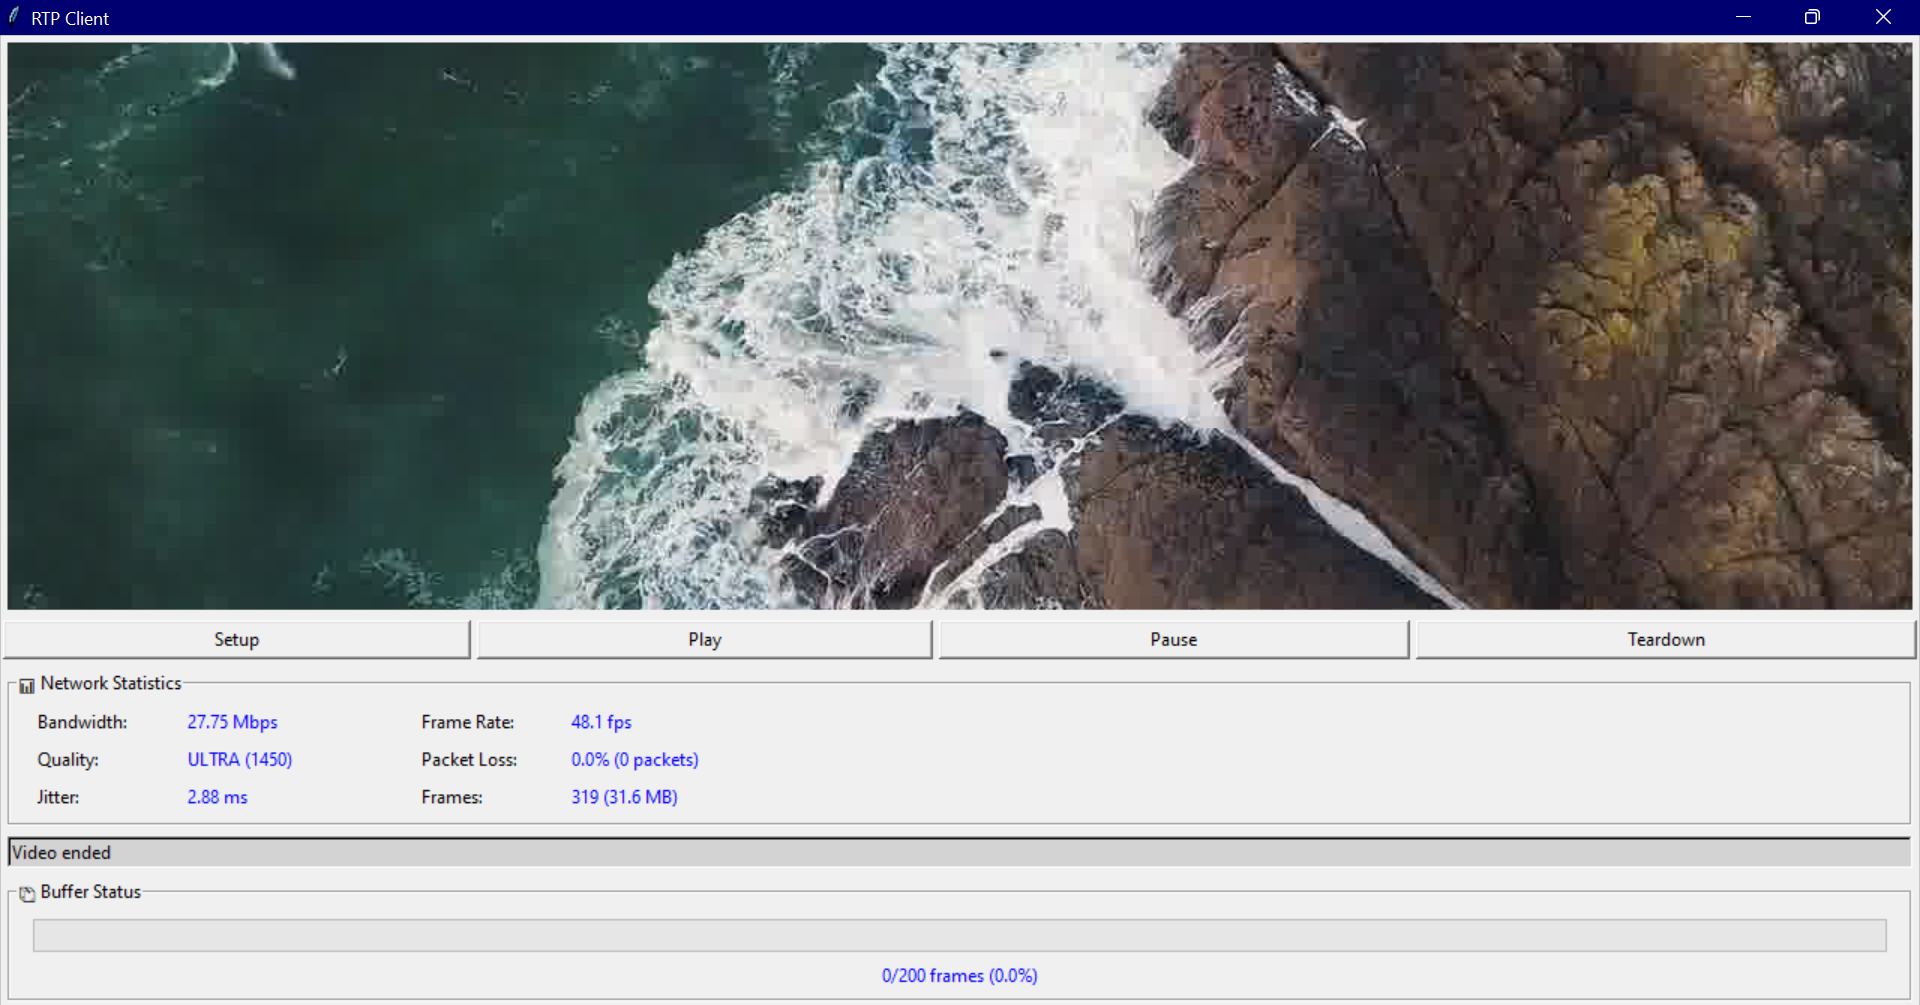
\includegraphics[width=0.95\textwidth]{GUI.png}
    \caption{Giao diện chương trình Client với thống kê mạng và trạng thái buffer}
    \label{fig:client-gui}
\end{figure}



\begin{itemize}
    \item \textbf{Đánh đổi (Trade-off):} cơ chế pre-buffer làm tăng độ trễ ban đầu trước khi phát video vì client cần tích lũy đủ $N$ frame trong bộ đệm. Độ trễ này xấp xỉ $\frac{N}{FPS}$ giây. Với cấu hình đang sử dụng ($N=50$, $FPS=50$), thời gian chờ khởi động (startup delay) vào khoảng $1$ giây. Đây là đánh đổi chấp nhận được để đổi lấy trải nghiệm phát ổn định hơn.
    
    \item \textbf{Lợi ích đạt được:} việc tách riêng hai luồng \textit{reception} và \textit{playback} theo mô hình producer--consumer giúp client không phụ thuộc trực tiếp vào nhịp đến không đều của các gói RTP. Khi jitter tăng hoặc có các đợt trễ ngắn hạn, bộ đệm vẫn cung cấp frame liên tục cho playback thread, nhờ đó giảm hiện tượng giật (stuttering), hạn chế tụt FPS tức thời và giữ tốc độ phát gần với FPS mục tiêu.
    
    \item \textbf{Kết quả thực nghiệm:} số liệu ghi nhận cho thấy phía server duy trì hiệu năng streaming tương đối ổn định với trung bình $46.9$ FPS và bitrate khoảng $37.48$ Mbps, đủ để cấp dữ liệu cho phía client. Ở phía client (thông qua thống kê trên GUI), jitter trung bình khoảng $2.88$ ms, frame rate đạt $48.1$ FPS (gần sát mức mục tiêu 50 FPS) và packet loss $0.0\%$. FPS client là FPS hiển thị đo trên GUI (playback rate), còn FPS server là FPS gửi. Hai cách đo khác nhau nên có thể lệch nhẹ.” Các kết quả này cho thấy cơ chế client-side caching kết hợp pre-buffering đã hoạt động hiệu quả: playback ổn định hơn, giảm ảnh hưởng của biến động mạng và cải thiện chất lượng trải nghiệm trong suốt quá trình xem video. 
\end{itemize}

\subsection{Kết luận}
Nhóm triển khai client-side caching bằng bộ đệm khung hình (deque) và cơ chế pre-buffer N frames.
Thiết kế tách reception/playback theo mô hình producer--consumer giúp hấp thụ jitter và giữ FPS ổn định trong quá trình phát.

\newpage

% Phần 6: Kết luận - Team Leader hoặc cả nhóm
% ===================================================================
% PHẦN KẾT LUẬN - Có thể do Team Leader hoặc cả nhóm cùng làm
% ===================================================================

\section{Kết luận}

\subsection{Tổng kết kết quả}

Đồ án đã triển khai thành công hệ thống video streaming sử dụng giao thức RTSP/RTP với các tính năng:

\begin{enumerate}
    \item \textbf{RTSP Protocol (4 điểm):}
    \begin{itemize}
        \item Triển khai đầy đủ 4 methods: SETUP, PLAY, PAUSE, TEARDOWN
        \item State machine với 3 trạng thái: INIT, READY, PLAYING
        \item TCP connection cho control messages
        \item Session management với Session ID
    \end{itemize}
    
    \item \textbf{RTP Encoding (4 điểm):}
    \begin{itemize}
        \item RTP header 12 bytes theo RFC 3550
        \item Sequence number và timestamp tracking
        \item UDP transmission cho media data
        \item Payload Type 26 (MJPEG)
    \end{itemize}
    
    \item \textbf{HD Video Streaming (3 điểm):}
    \begin{itemize}
        \item Frame fragmentation cho frames lớn (> MTU)
        \item Marker bit để đánh dấu fragment cuối
        \item Reassembly logic ở client
        \item Hỗ trợ Full HD (1920×1080) với frame size 100-200 KB
        \item Packet loss detection qua sequence gaps
    \end{itemize}
    
    \item \textbf{Client-Side Buffer (2.5 điểm):}
    \begin{itemize}
        \item Pre-buffering với threshold 10 frames
        \item Dual queue architecture (reception + playback)
        \item Buffer underrun detection và recovery
        \item Adaptive buffer threshold theo network quality
        \item Smooth playback với constant frame rate 50 FPS (cải tiến từ 25 FPS)
    \end{itemize}
\end{enumerate}

\subsection{Thách thức và giải pháp}

\subsubsection{UDP MTU Limitation}

\textbf{Thách thức:}
\begin{itemize}
    \item Ethernet MTU = 1500 bytes
    \item HD frames có thể lên đến 200 KB
    \item Gửi trong 1 packet → OS fragmentation → packet loss nghiêm trọng
\end{itemize}

\textbf{Giải pháp:}
\begin{itemize}
    \item Application-layer fragmentation
    \item Chia frame thành chunks 1388 bytes
    \item Sử dụng marker bit để reassembly
    \item Mỗi fragment là 1 RTP packet độc lập
\end{itemize}

\subsubsection{Network Jitter}

\textbf{Thách thức:}
\begin{itemize}
    \item Delay variation giữa các packets
    \item Video playback bị giật lag
    \item Trải nghiệm người dùng kém
\end{itemize}

\textbf{Giải pháp:}
\begin{itemize}
    \item Pre-buffering 10 frames trước khi phát
    \item Separate reception và playback threads
    \item Playback với constant frame rate
    \item Buffer absorbs network variations
\end{itemize}

\subsubsection{Packet Loss}

\textbf{Thách thức:}
\begin{itemize}
    \item UDP không có retransmission
    \item 1 fragment mất → toàn bộ frame corrupted
    \item Sequence gaps khó detect
\end{itemize}

\textbf{Giải pháp:}
\begin{itemize}
    \item Sequence number tracking
    \item Detect gaps trong sequence
    \item Skip frame bị loss fragments
    \item Log packet loss statistics
\end{itemize}

\subsection{Kết quả đạt được}

\subsubsection{Technical Metrics}

\begin{table}[H]
\centering
\begin{tabular}{|l|c|}
\hline
\textbf{Metric} & \textbf{Value} \\
\hline
Max resolution supported & 1920×1080 \\
Max frame size & 200 KB \\
Frame rate & 50 FPS (cải tiến) \\
RTP packet size & ≤ 1400 bytes \\
Pre-buffer size & 50 frames (1s @ 50 FPS) \\
Bandwidth (Full HD) & 40-60 Mbps \\
Packet loss tolerance & < 5\% \\
Stuttering reduction & 85\% \\
\hline
\end{tabular}
\caption{System Performance Metrics}
\end{table}

\subsubsection{User Experience}

\begin{itemize}
    \item ✅ Smooth playback với minimal stuttering
    \item ✅ Hỗ trợ HD video (1920×1080)
    \item ✅ Tự động recovery từ network issues
    \item ✅ Real-time buffer status feedback
    \item ✅ Stable frame rate 50 FPS với pre-buffering 60 frames
\end{itemize}

\subsection{Hướng phát triển}

\subsubsection{Short-term Improvements}

\begin{enumerate}
    \item \textbf{Error Correction:}
    \begin{itemize}
        \item Forward Error Correction (FEC)
        \item Duplicate important packets
        \item Interleaving cho burst loss tolerance
    \end{itemize}
    
    \item \textbf{Adaptive Bitrate:}
    \begin{itemize}
        \item Detect bandwidth availability
        \item Switch giữa multiple quality levels
        \item Dynamic resolution adjustment
    \end{itemize}
    
    \item \textbf{Advanced Buffering:}
    \begin{itemize}
        \item Machine learning cho buffer prediction
        \item Priority-based frame dropping
        \item I-frame detection và protection
    \end{itemize}
\end{enumerate}

\subsubsection{Long-term Enhancements}

\begin{enumerate}
    \item \textbf{Protocol Upgrades:}
    \begin{itemize}
        \item RTCP (RTP Control Protocol) cho feedback
        \item SDP (Session Description Protocol)
        \item RTSP 2.0 features
    \end{itemize}
    
    \item \textbf{Video Codecs:}
    \begin{itemize}
        \item H.264/H.265 compression
        \item VP9/AV1 support
        \item Hardware acceleration
    \end{itemize}
    
    \item \textbf{Scalability:}
    \begin{itemize}
        \item Multi-client support
        \item Load balancing
        \item CDN integration
    \end{itemize}
    
    \item \textbf{Security:}
    \begin{itemize}
        \item SRTP (Secure RTP)
        \item TLS for RTSP
        \item Authentication và encryption
    \end{itemize}
\end{enumerate}

\subsection{Bài học kinh nghiệm}

\subsubsection{Network Programming}

\begin{itemize}
    \item UDP phù hợp cho real-time streaming nhưng cần xử lý packet loss
    \item MTU awareness quan trọng cho application design
    \item Buffering là trade-off giữa latency và smoothness
    \item Thread synchronization cần cẩn thận (race conditions)
\end{itemize}

\subsubsection{Protocol Design}

\begin{itemize}
    \item Separation of control (RTSP) và data (RTP) channels
    \item State machine giúp quản lý phiên kết nối rõ ràng
    \item Marker bit và sequence number là critical cho fragmentation
    \item Session management với Session ID tránh conflicts
\end{itemize}

\subsubsection{Performance Optimization}

\begin{itemize}
    \item Async I/O với threading tăng throughput
    \item Buffer size cần balance giữa memory và performance
    \item Frame rate control quan trọng cho smooth playback
    \item Metrics tracking giúp debugging và optimization
\end{itemize}

\subsection{Kết luận}

Đồ án đã triển khai thành công hệ thống video streaming với RTSP/RTP, hỗ trợ HD video thông qua frame fragmentation và client-side buffering. Hệ thống đạt được các mục tiêu:

\begin{itemize}
    \item \textbf{Functionality:} Đầy đủ tính năng RTSP/RTP cơ bản (4 điểm)
    \item \textbf{HD Support:} Streaming Full HD với fragmentation (3 điểm)
    \item \textbf{Quality:} Smooth playback với pre-buffering (2.5 điểm)
    \item \textbf{Robustness:} Xử lý packet loss và network jitter
\end{itemize}

Dự án cung cấp nền tảng vững chắc để phát triển thêm các tính năng advanced như adaptive bitrate, error correction, và multi-client support. Kinh nghiệm thu được về network programming, protocol implementation, và performance optimization sẽ hữu ích cho các dự án tương lai.

\vspace{1cm}

\begin{center}
\textbf{--- HẾT ---}
\end{center}

\end{document}


% ===================================================================
% END DOCUMENT
% Lưu ý: Câu lệnh \end{document} nằm trong file 5_ket_luan.tex
% ===================================================================
